%%%%%%%%%%%%%%%%%%%%%%%%%%%%%%%%%%%%%%%%%%%%%%%%%%%%%%%%%%%%%%%%%%%%%%%%%%%%%%%%%%%%
% Do not alter this block (unless you're familiar with LaTeX
\documentclass{article}
\usepackage[margin=1in]{geometry} 
\usepackage{amsmath,amsthm,amssymb,amsfonts, fancyhdr, color, comment, graphicx, environ}
\usepackage{xcolor}
\usepackage{mdframed}
\usepackage[shortlabels]{enumitem}
\usepackage{indentfirst}
\usepackage{hyperref}
\usepackage{algorithm2e}
\usepackage{pgfgantt}
\usepackage{tikz}
\usepackage{tikz-qtree}
\makeatletter
\@gtt@keydef{anyday}{none}
\@gtt@keydef{anyday offset}{1}
\@gtt@stylekeydef{anyday rule}{dashed, line width=1pt}
\@gtt@keydef{anyday label font}{\normalfont}
\@gtt@stylekeydef{anyday label node}{%
  anchor=north, font=\ganttvalueof{anyday label font}%
}

\newcount\gtt@anyday@slot

\newcommand\gantText[2]{%
  \gtt@tsstojulian{#1}{\gtt@anyday@slot}%
  \gtt@juliantotimeslot{\gtt@anyday@slot}{\gtt@anyday@slot}%
  \pgfmathsetmacro\y@upper{%
    \gtt@lasttitleline * \ganttvalueof{y unit title}%
  }%
  \pgfmathsetmacro\y@lower{%
    \gtt@lasttitleline * \ganttvalueof{y unit title}%
      + (\gtt@currentline - \gtt@lasttitleline - 1)%
      * \ganttvalueof{y unit chart}%
  }%
  \pgfmathsetmacro\x@mid{%
    (\gtt@anyday@slot - 1 + \ganttvalueof{anyday offset})%
      * \ganttvalueof{x unit}%
  }%
  \node [/pgfgantt/anyday label node]
     at (\x@mid pt, \y@lower pt) {#2};
}
\makeatother
\newtheorem{theorem}{Theorem}
\hypersetup{
    colorlinks=true,
    linkcolor=blue,
    filecolor=magenta,      
    urlcolor=blue,
}


\pagestyle{fancy}


\newenvironment{problem}[2][Problem]
    { \begin{mdframed}[backgroundcolor=gray!20] \textbf{#1 #2} \\}
    {  \end{mdframed}}

% Define solution environment
\newenvironment{solution}
    {\textit{Solution:}}
    {}

\renewcommand{\qed}{\quad\qedsymbol}

% prevent line break in inline mode
\binoppenalty=\maxdimen
\relpenalty=\maxdimen

%%%%%%%%%%%%%%%%%%%%%%%%%%%%%%%%%%%%%%%%%%%%%
%Fill in the appropriate information below
\lhead{Pengju Zhang}
\rhead{CSC-421} 
\chead{\textbf{Assignment 4}}
%%%%%%%%%%%%%%%%%%%%%%%%%%%%%%%%%%%%%%%%%%%%%

\begin{document}

%problem 1
\begin{problem}{1}
\textbf{[50 pts]}
The greedy algorithm we described for the class scheduling problem is not the only greedy strategy we could have tried. For each of the following alternative greedy strategies, either prove that the resulting algorithm always constructs an optimal schedule, or describe a small input example for which the algorithm does not produce an optimal schedule. Assume that all algorithms break ties arbitrarily (that is, in a manner that is completely out of your control).
\begin{enumerate}
	\item Choose the course x that ends last, discard classes that conflict with x, and recurse.
	\item Choose the course x that starts first, discard all classes that conflict with x, and recurse.
	\item Choose the course x that starts last, discard all classes that conflict with x, and recurse.
	\item Choose the course x with shortest duration, discard all classes that conflict with x, and recurse.
	\item If no classes conflict, choose them all. Otherwise, discard the course with longest duration and recurse.
	\item If no classes conflict, choose them all. Otherwise, discard a course that conflicts with the most other courses and recurse.
	\item If any course x completely contains another course, discard x and recurse. Otherwise, choose the course y that ends last, discard all classes that conflict with y, and recurse.
\end{enumerate}
\end{problem}
\begin{solution}
\begin{enumerate}
	\item \mbox{}
	This doesn’t work.
	\newline
	\begin{ganttchart}[vgrid, hgrid]{1}{12}
		\gantttitle{Greedy Schedule Example}{12} \\
		\ganttbar{Task 1}{3}{3} 
		\ganttbar{}{5}{5} 
		\ganttbar{}{7}{7} 
		\ganttbar{}{9}{9} \\
		\ganttbar{Task 2}{2}{10}  \\
		\gantText{6}{$Timeline$}
	\end{ganttchart}
	\newline
	Given the input above, the greedy algorithm chooses the single long course, but the optimal schedule contains all the short courses. 
	\item \mbox{}
	This doesn’t work, same as part (1).
	\item \mbox{}
	This greedy algorithm works.
	\newline
	Let x be the course that starts last. Let $S$ be any schedule that does not contain $x$, and let $z$ be the last course in $S$. Because $x$ starts last, we have $S[z] < S[x]$. Thus $F[i] < S[z] < S[x]$ for every other class $i$ in $S$, which implies that $S' = S - z + x$ is still a valid schedule, containing the same number of classes as $S$. In particular, if $S$ is an optimal schedule, then $S'$ is an optimal schedule containing $x$.
	\item \mbox{}
	This doesn’t work.
	\newline
	\begin{ganttchart}[vgrid, hgrid]{1}{12}
		\gantttitle{Greedy Schedule Example}{12} \\
		\ganttbar{Task 1}{5}{8} \\
		\ganttbar{Task 2}{2}{5}  
		\ganttbar{}{8}{11} \\
		\gantText{6}{$Timeline$}
	\end{ganttchart}
	\newline	
	Given the input above, this greedy algorithm chooses the single course in the middle, but the optimal schedule contains the other two courses.
	\item \mbox{}
	This doesn’t work, same as part (4).
	\item \mbox{}
	This doesn’t work.
	\newline
	\begin{ganttchart}[vgrid, hgrid]{1}{15}
		\gantttitle{Greedy Schedule Example}{15} \\
		\ganttbar{Task 1}{5}{7} 
		\ganttbar{}{9}{11} \\
		\ganttbar{Task 2}{3}{6}  
		\ganttbar{}{8}{8}
		\ganttbar{}{10}{13}\\
		\ganttbar{Task 3}{2}{5}  
		\ganttbar{}{7}{9}
		\ganttbar{}{11}{14}\\
		\ganttbar{Task 4}{1}{3}  
		\ganttbar{}{5}{7}
		\ganttbar{}{9}{11}
		\ganttbar{}{13}{15}\\
		\gantText{6}{$Timeline$}
	\end{ganttchart}
	\newline
	Given the input above, this greedy algorithm would discard one of the courses in the middle of the bottom row, which has only five conflicts, and thus would return a schedule containing only three courses. But the optimal schedule contains four courses. 
	\item \mbox{}
	This greedy algorithm works.
	\newline
	Let $S$ be any valid schedule that contains $x$. Then $S - x + y$ is another valid schedule of the same size. If no course contains any other course, then the class that ends last is also the class that starts last.	
\end{enumerate}
\end{solution}

%problem 2
\newpage
\begin{problem}{2}
\textbf{[15 pts]} 
Construct a Huffman code for the following set of characters and their frequencies that are based on the first 8 Fibonacci numbers:
\newline
a : 1; b : 1; c : 2; d : 3; e : 5; f : 8; g : 13; h : 21.
\end{problem}
\begin{solution}
\newline
\usetikzlibrary{trees}
\begin{tikzpicture}[iv/.style={draw, circle,minimum size=20pt,inner
sep=0pt,text=black},ev/.style={draw,rectangle,minimum
size=24pt,inner sep=0pt,text=black}]
\node[iv]{54}
  child {node[iv]{33}
         child {node[iv]{20}  
                child {node[iv]{12}
                       child {node[iv]{7}
                              child {node[iv]{4}
                              	child {node[iv]{2}
					child {node[ev]{a: 1}}
					child {node[ev]{b: 1}}
				}
				child {node[ev]{c: 2}}
                              }
                              child {node[ev]{d: 3}}
                             }
                       child {node[ev]{e: 5}}
                      }
                child {node[ev]{f: 8}}
                }
         child [missing]
         child {node[ev]{g: 13}
               }      
        }
  child [missing]
  child [missing]
  child {node[ev]{h: 21}};
\end{tikzpicture}
\newline
As we can see the tree is one long limb with leaves n = hanging off. This is true for Fibonacci weights in general, because the Fibonacci the recurrence is implies that
	\begin{equation}
		F_{n + 2}= \sum_{i = 0}^{n} F_{i} + 1
	\end{equation}
\end{solution}

%problem 3
\newpage
\begin{problem}{3}
\textbf{[20 pts]}
An independent set in a graph $G$ is a set of vertices $I$ in $G$ such that no two vertices in $I$ are adjacent (neighbors). The maximum independent set problem is, given a graph $G$, to compute an independent set in $G$ of maximum size (maximum number of vertices). Pinocchio claims that he has a greedy algorithm that solves the maximum independent set problem. Pinocchio’s algorithm works as follows. The algorithm initializes the set $I$ to the empty set, and repeats the following steps: Pick a vertex in the graph with the minimum degree, add it to the set $I$, and remove it and all the vertices adjacent to it from the graph. The algorithm stops when the graph is empty. Does Pinocchio’s greedy algorithm always produces a maximum independent set? Prove your answer (if it does, give a proof; if it does not, give a counter example, that is, a graph on which Pinocchio’s algorithm does not produce a maximum independent set).
\end{problem}
\begin{solution}
\newline
Pinocchio’s algorithm is not guaranteed to find a maximum independent set.
\newline
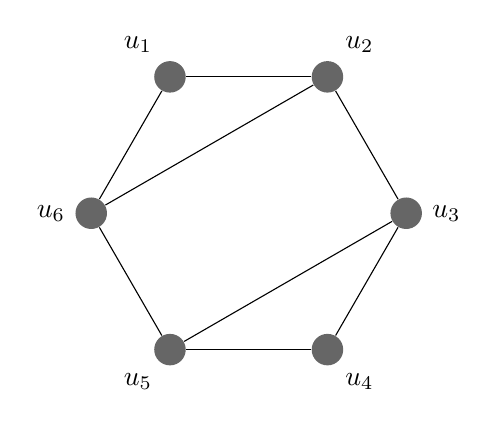
\begin{tikzpicture}[roundnode/.style={circle, fill=black!60, inner sep=0pt, minimum size=4mm}]
   	\foreach \i [count=\ni] in {120, 60, ..., -180}
       		\node[roundnode, label=\i:{$u_\ni$}] at (\i:2cm) (u\ni) {};
        	   	\draw[-] (u1) -- (u6);
            	\draw[-] (u2) -- (u6);
            	\draw[-] (u3) -- (u5);
            	\draw[-] (u4) -- (u5);
            	\draw[-] (u5) -- (u6); 
		\draw[-] (u4) -- (u3); 
		\draw[-] (u1) -- (u2); 
		\draw[-] (u2) -- (u3); 
\end{tikzpicture}
\newline
It is not no hard to tell the maximum independent set would be $[u_1, u_3, u_5]$ or $[u_4, u_2, u_6]$. Follow by Pinocchio’s algorithm we have to either add $u_1$ or $u_4$ into set $I$ since they both have least degree of 2. Assume we start at vertex $u_1$ we have to remove $u_6$ and $u_2$, this result to a triangle graph among $u_3$, $u_4$ and $u_5$, due to Pinocchio’s algorithm we can only keep one of them into set $I$.
Consequently, Pinocchio’s algorithm result $[u_1, u_3]$, $[u_1, u_4]$, $[u_1, u_5]$ are contradict to our actual result.
\end{solution}

%problem 4
\newpage
\begin{problem}{4}
\textbf{[15 pts]} 
Professor Gekko has always dreamed of inline skating across North Dakota. He plans to cross the state on highway U.S. 2, which runs from Grand Forks, on the eastern border with Minnesota, to Williston, near the western border with Montana.
\newline
The professor can carry two liters of water, and he can skate m miles before running out of water. (Because North Dakota is relatively flat, the professor does not have to worry about drinking water at a greater rate on uphill sections than on flat or downhill sections.) The professor will start in Grand Forks with two full liters of water. His official North Dakota state map shows all the places along U.S. 2 at which he can refill his water and the distances between these locations.
\newline
The professor’s goal is to minimize the number of water stops along his route across the state. Give an efficient algorithm by which he can determine which water stops he should make. Prove that your strategy yields an optimal solution, and give its running time.
\end{problem}
\begin{solution}
	\begin{algorithm}
		\SetKwProg{Def}{def}{:}{}
		\Def{MinWaterStop(availableSpot)}{
			distance $\gets$ 0;\\
			\For {each spot in order} {
				\If{distance + dstanceToNextSpot $>$ 2 mile} {
					markCurrentSpot();\\
					numberOfWaterSpot++;\\
					distance = 0;
				}
				\Else {
					distance += distanceToNextSpot;
				}
			}
			return markedSpot;
		}
	\end{algorithm}
	\newline
	By following the algorithm shown above, the professor will not make a water stop if the distance from last refill to the upcoming refill is less than 2 miles. He will stop for refill only when he cannot reach the next spot at any point. That is, it holds suboptimal property all along, with m minimal stops in total. Assuming that there is a better solution with m - 1 stops, it is impossible to finish the section after the omitted spot. Therefore, the algorithm is optimal. And its running time is $O(n)$ where n is the number of available spots.
\end{solution}
\end{document}